\chapter{Building Correlation Between Filters in Convolutional Neural Networks}

{\small \textbf{Authors}\\
Hanli Wang, \textit{Senior Member, IEEE}, Peiqiu Chen, and Sam Kwong, \textit{Fellow, IEEE}\\ \\
IEEE TRANSACTIONS ON CYBERNETICS\\VOL. 47, NO. 10, OCTOBER 2017}

\section{Proposed Method}

In this paper we will present a particular approach that aims at improving performance in CNNs through some observations on filters. It has already been explained how convolution generally works. Recall that we are looking for features to extract by learning some weights. The main idea here is to propose two different types of correlative filters. They are respectively \textit{static correlative filters} (SCFs) and \textit{parametric correlative filters} (PCFs). Before of going any further it would be worth understanding the basic idea for this study. Basically, it turns out from the paper that there is a link with neuroscience. More specifically, it has been observed that there are cells more sensitive to the light and others more sensitive to the darkness. Taking inspiration from that, we want to understand whether or not there is any connection between this idea and the way filters extract features from images in CNNs. Having said that, let us talk about the two proposed correlative filters approaches. As far as static correlative filters, four kinds of these filters are proposed and they are: opposite correlation, rotary correlation, scaling correlation and translational correlation. The idea is that we have some filters divided into \textit{master} and \textit{dependent} filters. If we let $m_{i,j}$ be the master and $d_{i,j}$ be the dependent filter, we end up with a few results. For instance, as concerns the \textit{opposite correlation} we will have that $d_{i,j} = -m_{i,j}$. In fact, if we take a look at letters (a) and (b) of Figure \ref{fig:02_1}, it is quite clear that in the dependent filter we obtain the exact opposite of the master filter. As far as the rotary correlation, for computational convenience, it has been considered only a rotation of 90°. On scaling correlation, a scaling equation is applied in order to reduce the size along both dimensions, width and height. Finally, as regards the translational correlation, which seems to be more complex, two filter have been used and they represent the part of the filter that goes upward and the other one that goes downward.\\

\begin{figure}[h!]
    \centering
    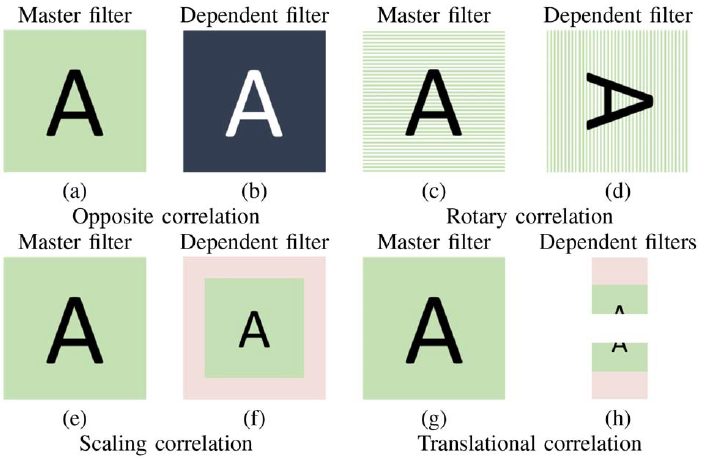
\includegraphics[scale=0.60]{images/02_1.png}
    \caption{Four kinds of proposed SCFs}
    \label{fig:02_1}
\end{figure}

\FloatBarrier

Another aspect that has been presented is how correlative filters are connected. It turns out that there are two strategies. They are the \textit{cross-map} connection and the \textit{within-map} connection. The first one is used with opposite and rotary correlations, while the second one is used on scaling and translational correlations. So far, it has been only said that there is a master and a dependent filter but it has not been shown how they work together. In Figures \ref{fig:02_2} and \ref{fig:02_3} is given an illustration of cross-map and within-map connections.

\begin{figure}[h!]
    \centering
    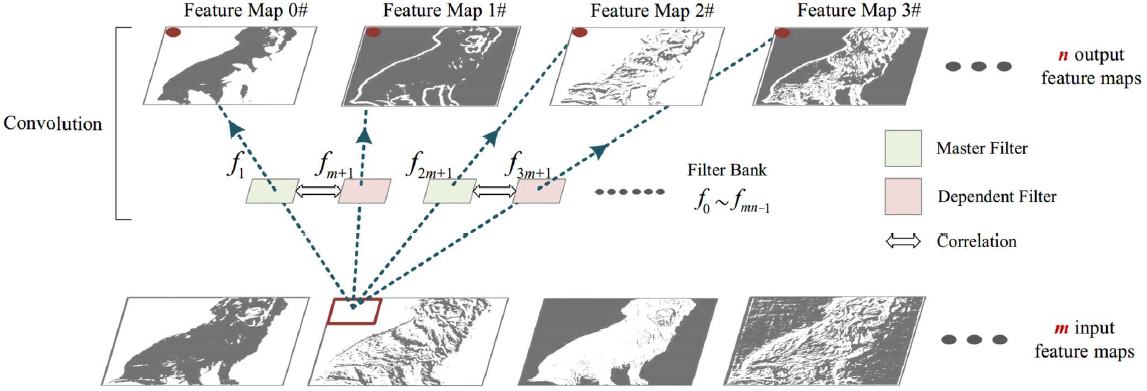
\includegraphics[scale=0.50]{images/02_2.png}
    \caption{Cross-map connection.}
    \label{fig:02_2}
\end{figure}

\FloatBarrier

\begin{figure}[h!]
    \centering
    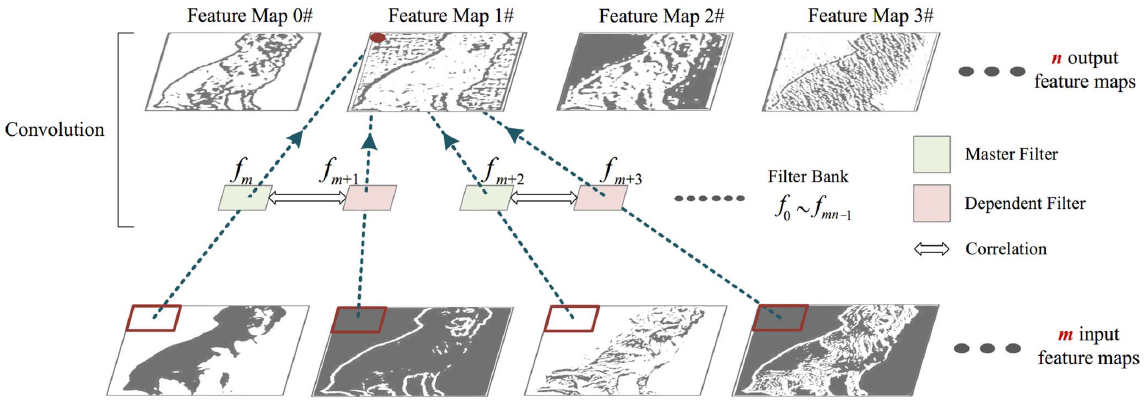
\includegraphics[scale=0.50]{images/02_3.png}
    \caption{Within-map connection.}
    \label{fig:02_3}
\end{figure}

\FloatBarrier

The main difference between the two is that in the cross-map connection we have a master that shares its feature map with a dependent filter but they refer to different output features. Instead, in the within-map connection, the master comes from a different input feature map but winds up in the same output feature map of other filters.\\ \\
Finally, there are parametric correlative filters (PCFs). They have been proposed in case we have not considered other correlations. The basic idea here is to use a correlation matrix which is gradually updated after the backward propagation. In fact it is possible to define this type of correlative filter like a fully-connected layer in an ordinary NN, so it follows the same logic. An illustration of how this correlative filter works is given in Figure \ref{fig:02_4}.\\

\begin{figure}[h!]
    \centering
    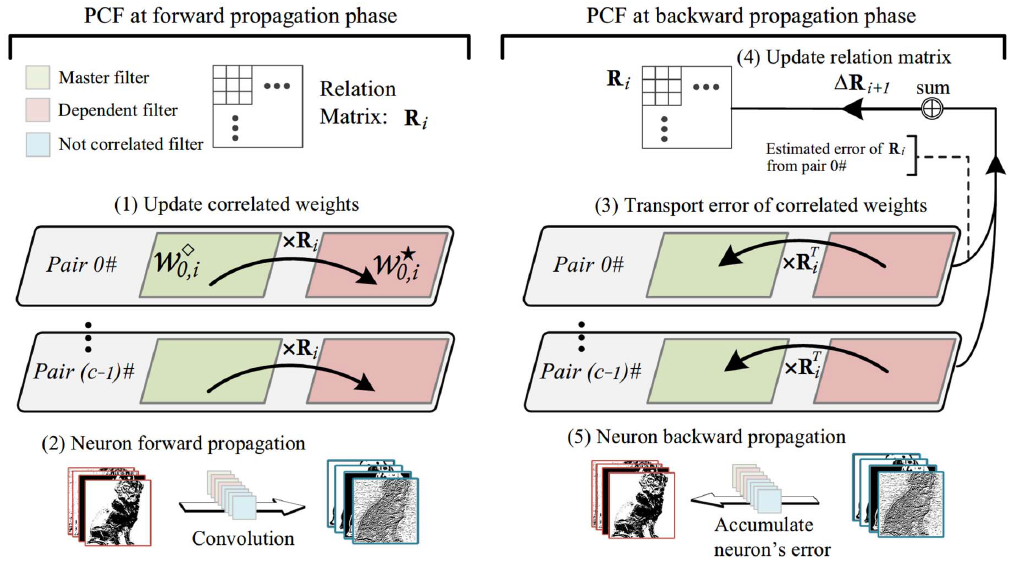
\includegraphics[scale=0.55]{images/02_4.png}
    \caption{PCFs training.}
    \label{fig:02_4}
\end{figure}

\FloatBarrier

\section{Experimental Results}

As far as the experimental results, five datasets have been used and they are: CIFAR10 \citep{CIFAR10and100}, CIFAR100 \citep{CIFAR10and100}, MNIST \citep{MNIST}, STL-10 \citep{STL10} and SVHN \citep{SVHN}. On some tests, data augmentation is performed. As it is the first paper in which we find this tecnique, it is worth saying a few words about it. Data augmentation is usually used when we do not have large datasets and we want to prevent overfitting as well. Basically, by performing simple operations such as cropping, flipping, etc. we can add more images for the same subject into our dataset. By doing so, if we run into some changes in light intensity for the given input image, we will still be able to classify correctly that image. Data augmentation is very useful and it allows to have better results on classification tasks and for this reason is widely used. Another tecnique applied in this paper is a classical regularization tecnique such as the dropout. In the end, by adopting the model SCF+PCF, it turns out that very good results are obtained on dataset previously mentioned with and without data augmentation. 
